\subsection{V2I Communication}
\label{sec:design_and_implementation}
%%% image process 3 state machine
\begin{figure}[ht]
    \centering
    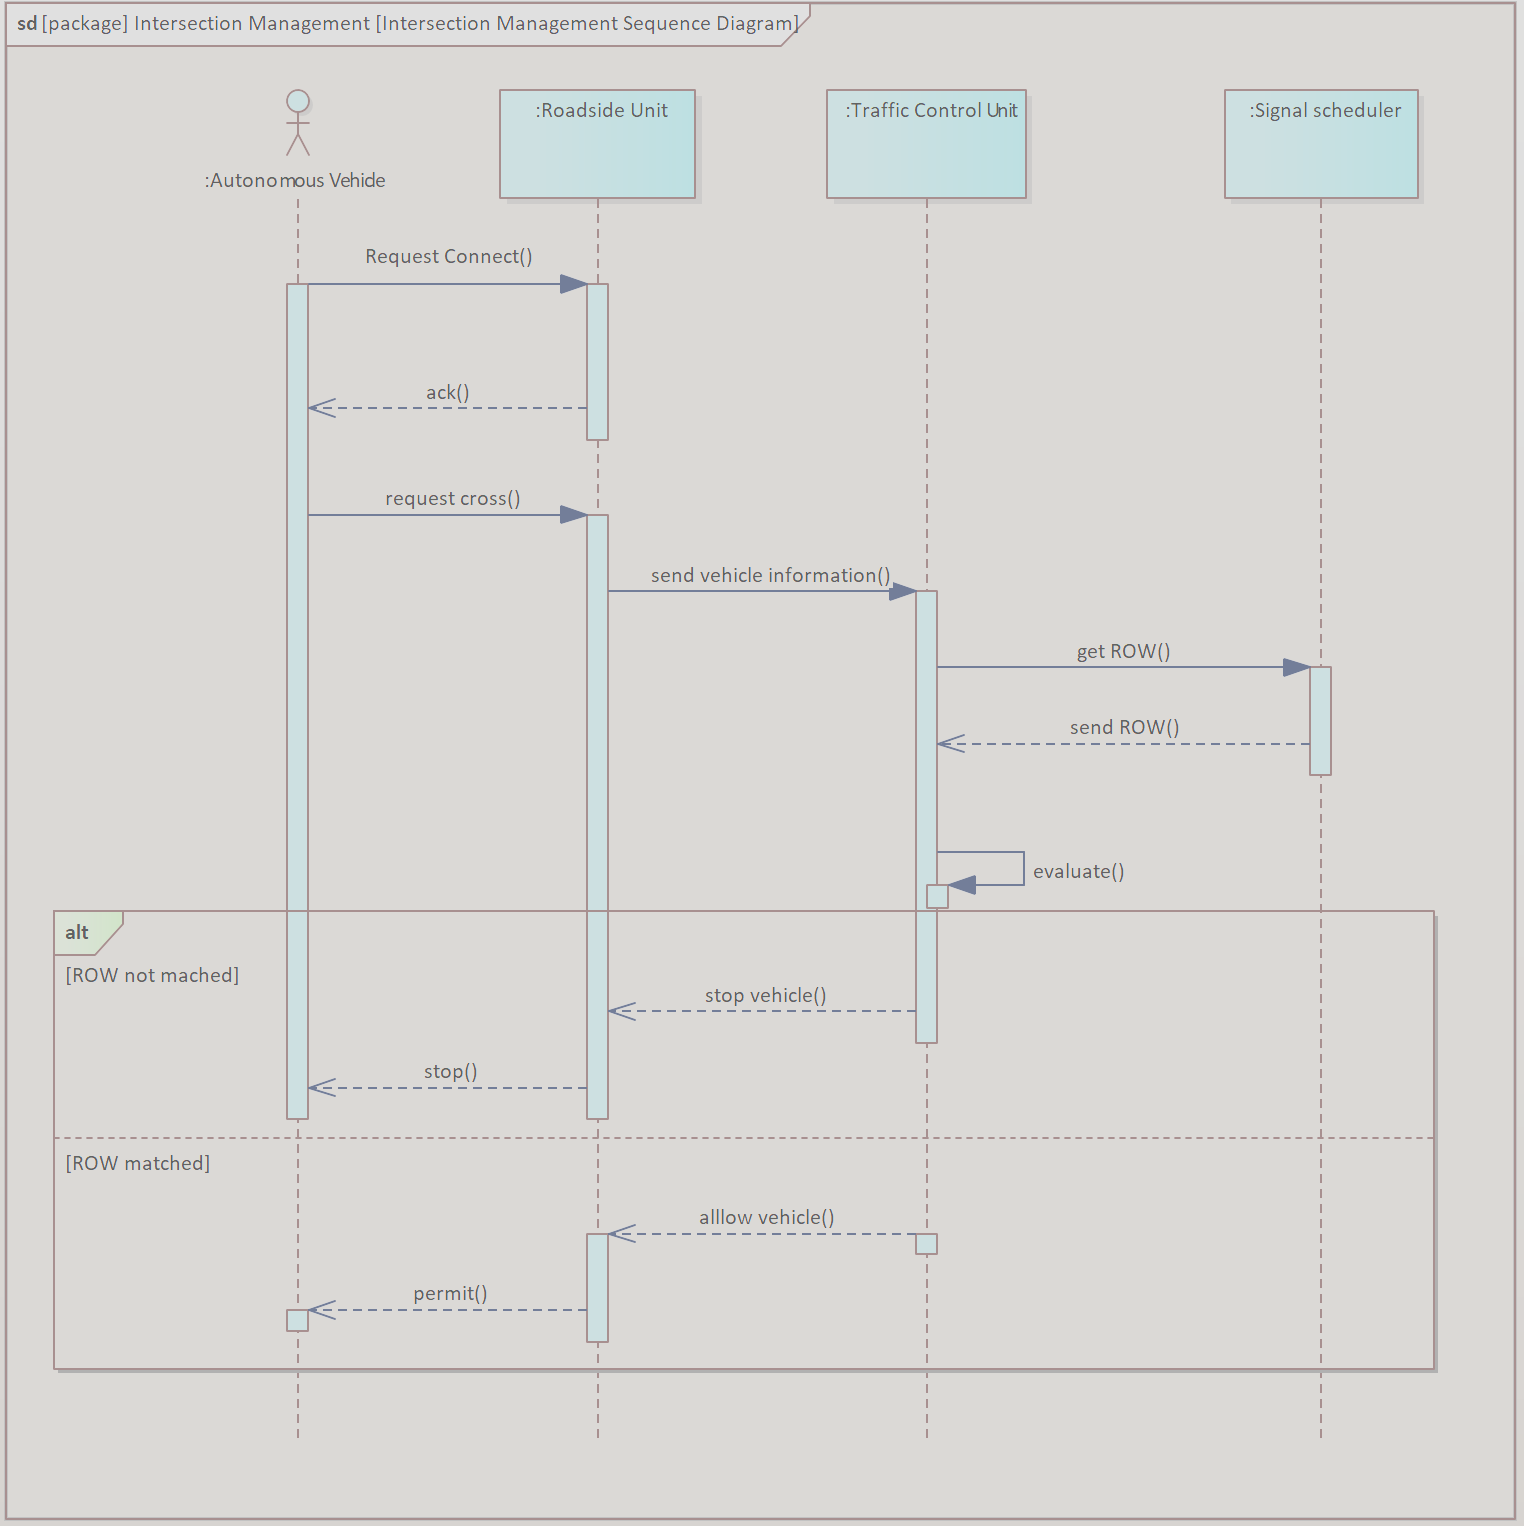
\includegraphics[width=0.5\textwidth]{images/intersection_management.png}
    \caption{Vehicle cross an intersection scenario }
    \label{img:intersection_management}
\end{figure}
 The Figure \ref{img:intersection_management} illustrates the process by which an autonomous vehicle requests permission to cross an intersection. The vehicle sends a request message to the nearest RSU, which acts as a relay between the vehicle and the TCU. The RSU forwards the request to the TCU, which is responsible for managing the traffic flow and signals at the intersection. The TCU consults with the Signal Scheduler, which is a module that determines the right of way (ROW) for each vehicle based on various factors, such as traffic density, priority, and safety. The Signal Scheduler returns the ROW status to the TCU, which then sends an instruction message to the RSU. The RSU relays the instruction to the vehicle, which can either proceed or stop depending on the ROW status. 

%%% image process 3 state machine
\begin{figure}[ht]
    \centering
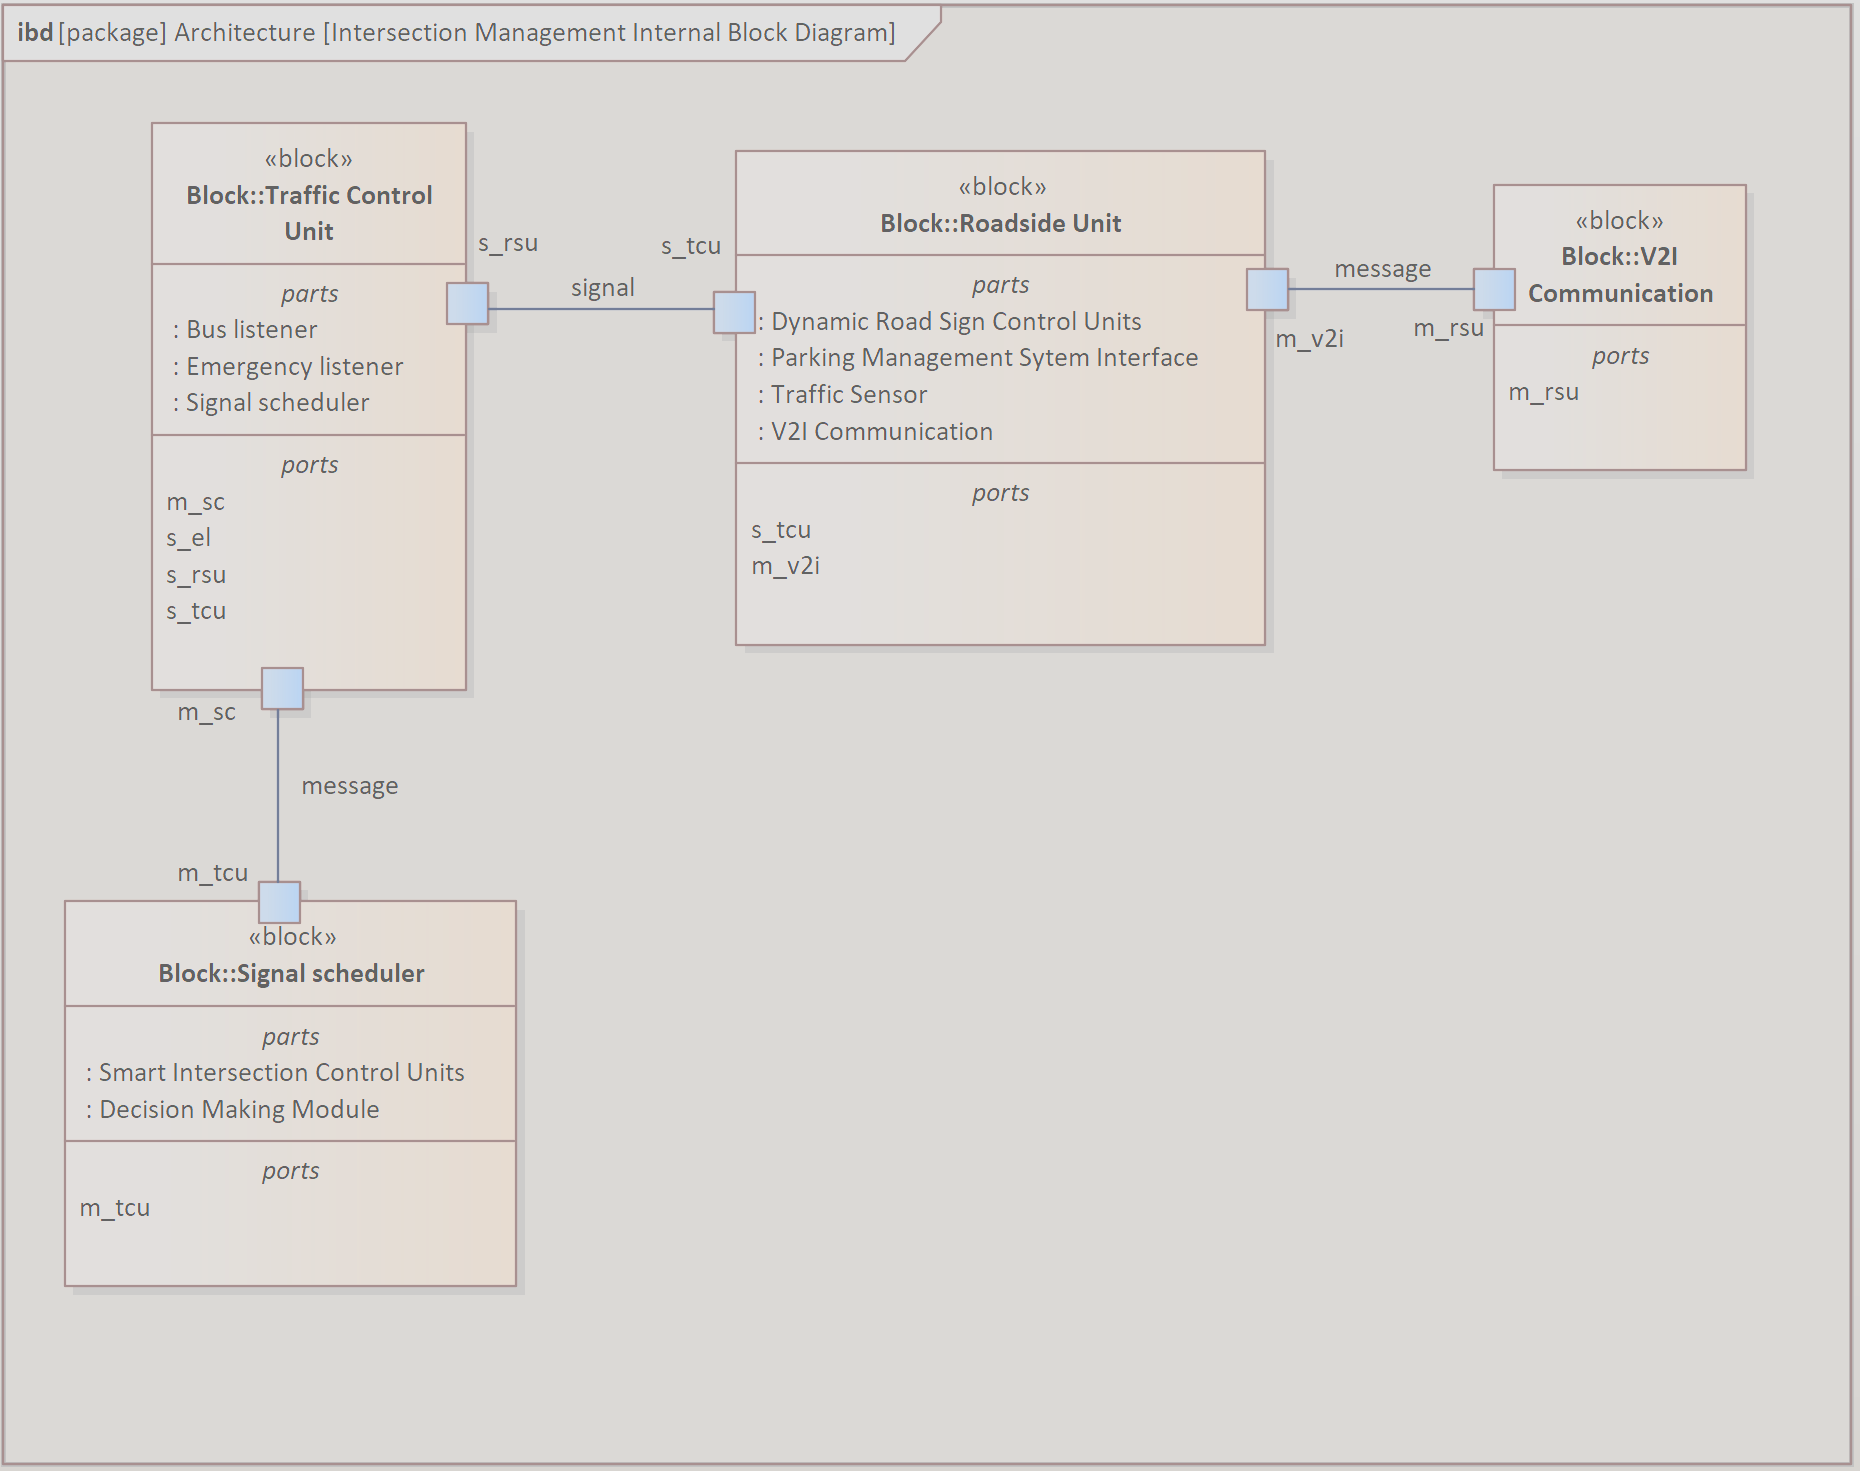
\includegraphics[width=0.5\textwidth]{images/v2i_ibd.png}
    \caption{System component interaction}
    \label{img:v2i_ibd}
\end{figure}

The architecture of the Intersection Management System consists of two main blocks: Traffic Control and Roadside Unit shown in Figure \ref{img:v2i_ibd}. The Traffic Control block encompasses the TCU and the Signal Scheduler, as well as other components, such as Emergency Listener, Signal scheduler and Smart Intersection Control Units, Decision Making Module. The Emergency Listener and  Signal Scheduler is an interface that allows emergency vehicles, such as ambulances and fire trucks, to override the normal traffic signals and gain priority access to the intersection. The Smart Intersection Control and Units Decision Making Module are components that implement advanced algorithms and logic to optimize the traffic flow and signals at the intersection. The Traffic Sensor is a component that validates the traffic and the instruction received from the TCU and executes the appropriate action. The communication between these blocks and components is facilitated by messages exchanged via ports, as indicated by the arrows in the diagram. This diagram provides a detailed view of the Intersection Management System’s architecture, and how it integrates different modules and interfaces to achieve safe and efficient navigation at the intersection.


\subsection{TCU Processor}
\label{sec:design_and_implementation}
%%% image process 3 state machine
\begin{figure}[ht]
    \centering
    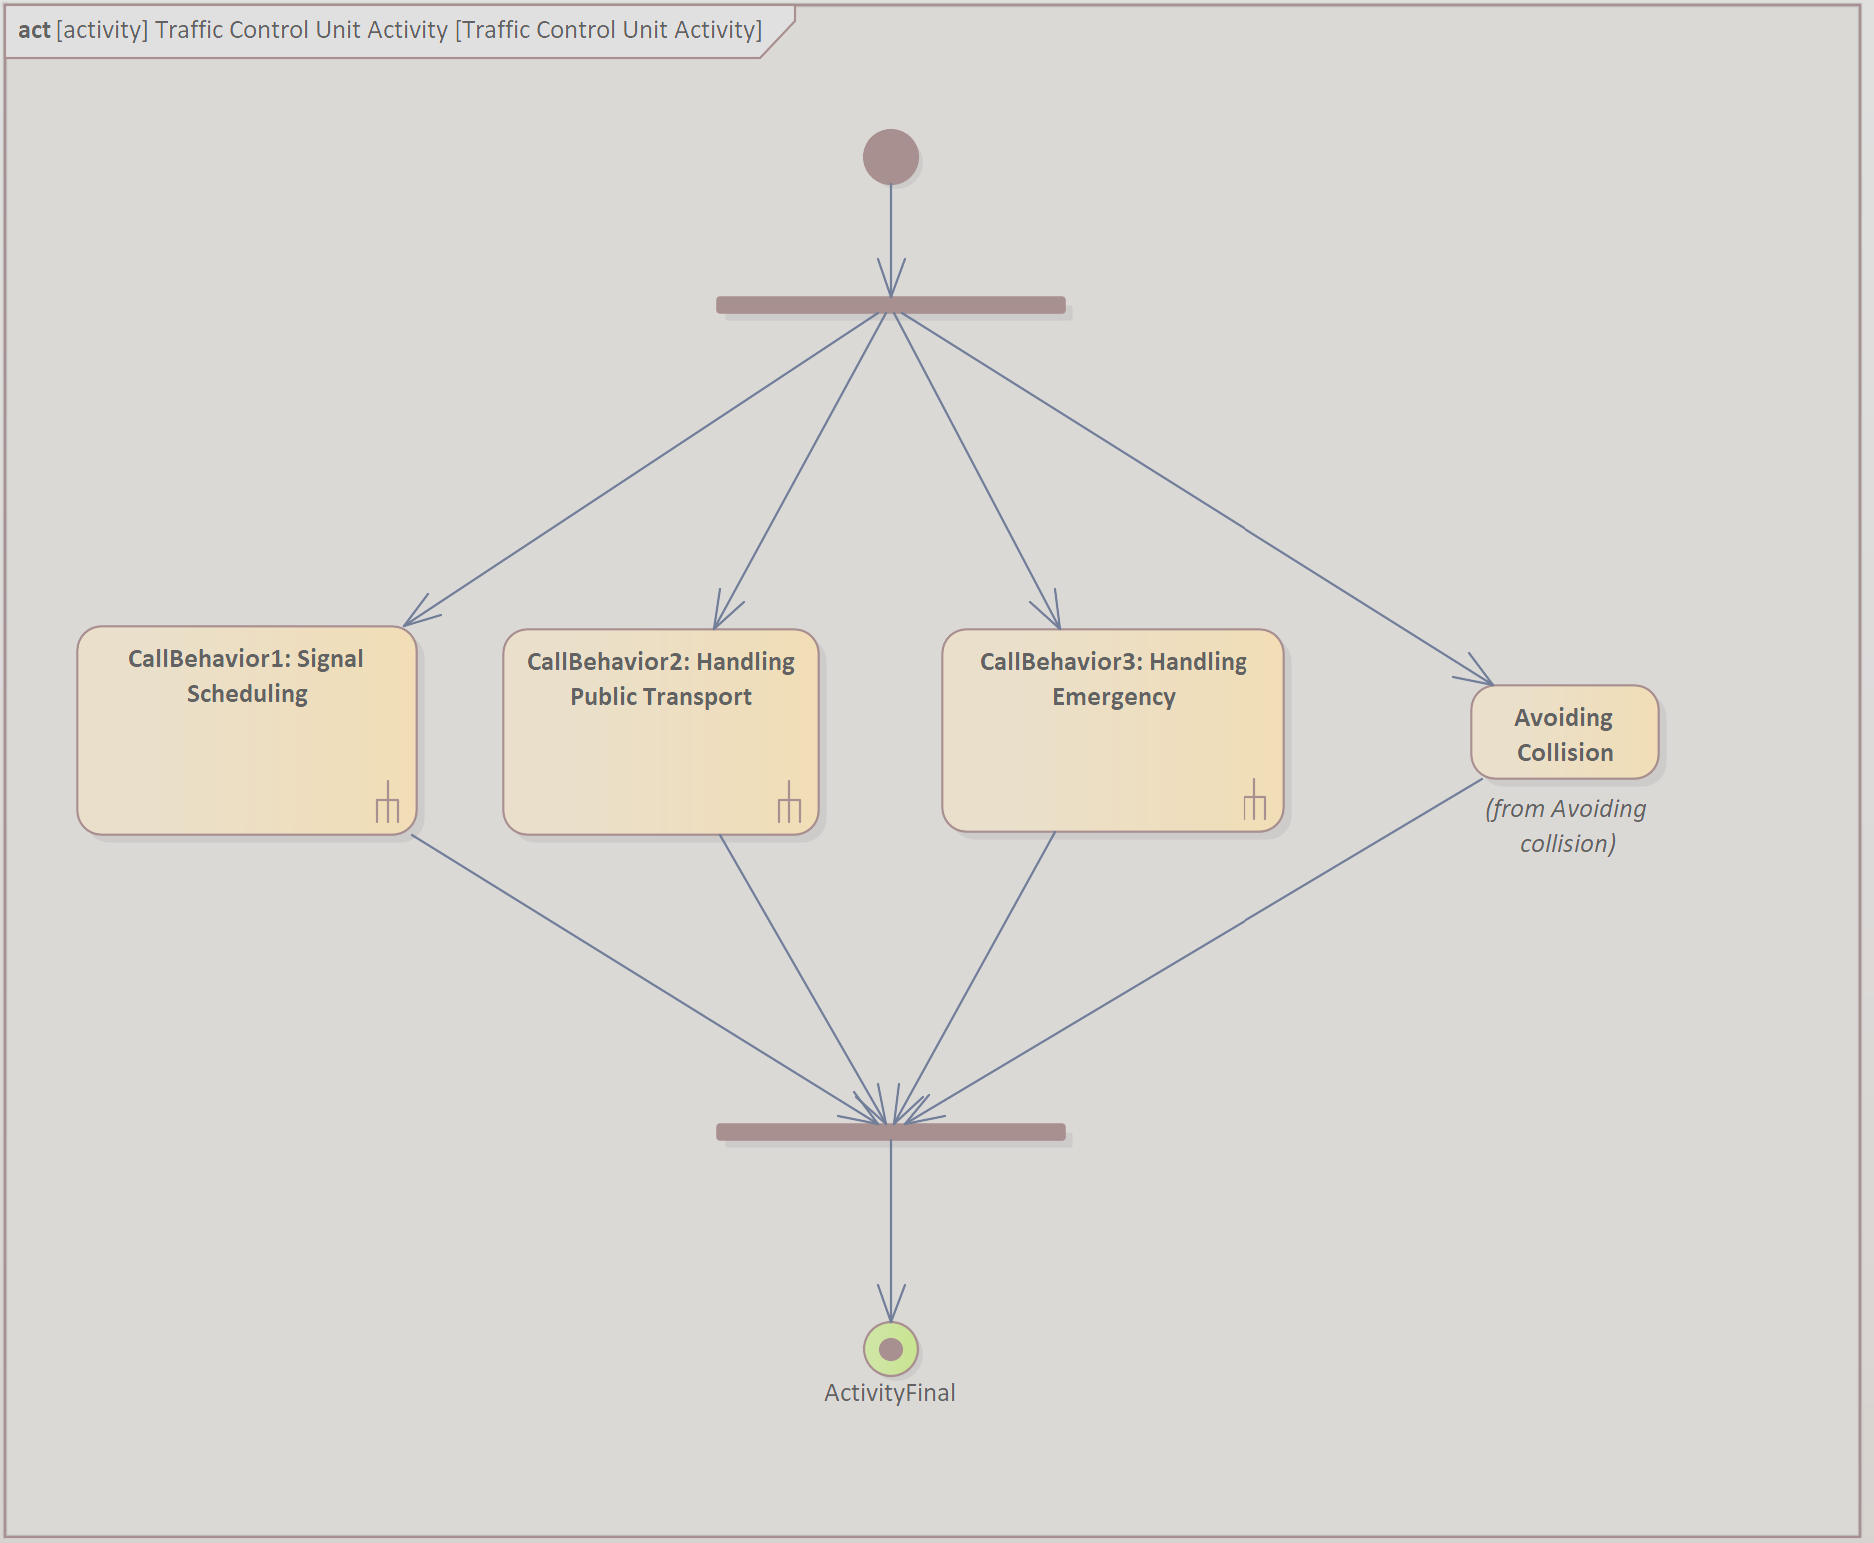
\includegraphics[width=0.5\textwidth]{images/tcu_process.png}
    \caption{Traffic Control Unit processes }
    \label{img:tcu_process}
\end{figure}
The Traffic Control Unit (TCU) shown in Figure \ref{img:tcu_process} is the key component for our networked traffic control system, and is responsible for optimizing traffic flow and improving road safety. It manages traffic lights to alleviate congestion, prioritizes public transportation to ensure schedule adherence, handles emergencies by redirecting traffic and assisting emergency vehicles, and uses sensor data to avoid collisions. The TCU receives data from the RSU first and then performs three major functions, which we are :
\begin{itemize}
\item Signal Scheduling ensures that vehicles operate smoothly and efficiently. Its goal is to reduce wait times and congestion through efficient traffic light coordination.
\end{itemize}
\begin{itemize}
\item Handling Public Transport: This process prioritizes buses and trams. The purpose is to ensure the timely flow and efficiency of public transportation.
\end{itemize}
\begin{itemize}
    \item Handling Emergency: This process focuses on rerouting traffic and prioritizing emergency vehicles. The goal is to guarantee that emergency vehicles arrive at their destinations quickly.


\end{itemize}

 

\subsection{RSU Behaviour}
\label{sec:design_and_implementation}
%%% image process 3 state machine
\begin{figure}[ht]
    \centering
    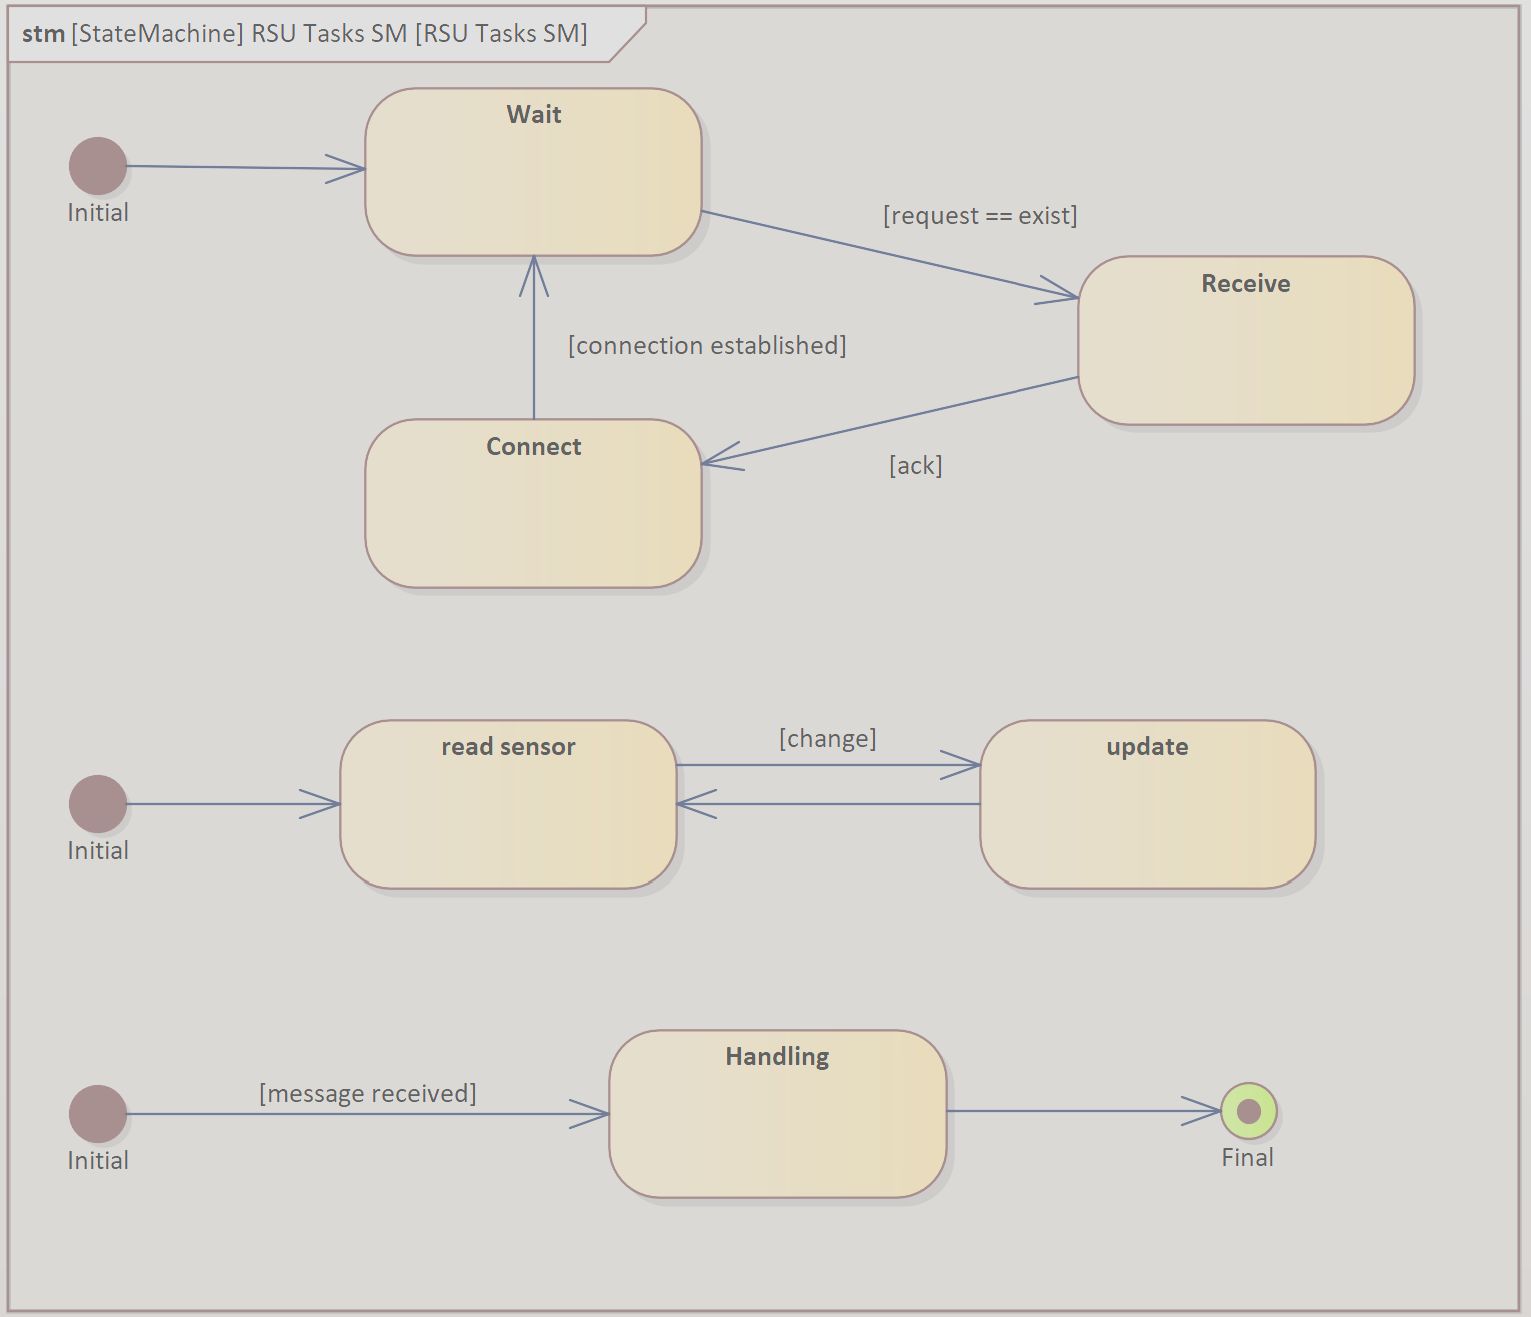
\includegraphics[width=0.5\textwidth]{images/rsu_state_machine.png}
    \caption{RSU Processes }
    \label{img:rsu_state_machine}
\end{figure}
RSUs use three state machines, as shown in Figure \ref{img:rsu_state_machine}, to manage traffic efficiently.
The first state machine manages communication. In the 'Wait' mode, the RSU awaits incoming requests from cars or (TCUs). When it senses a request, it enters the 'Connect' state to establish communication with the requester. After successfully connecting, it enters the 'Receive' stage, where it is prepared to receive data or commands from the connected entity. The second state machine focuses on sensor inputs. The RSU continuously monitors sensor data, such as traffic conditions or environmental information. When it detects significant changes in this data, it enters the 'Update' state. The third handles message processing, transitioning from a passive to a 'Handling' state upon message receipt in order to process and act on the data. These techniques allow RSUs to effectively manage communication, sensor data, and messages, which is critical for reacting to and controlling real-time traffic circumstances.





